\documentclass[a4paper,12pt]{article}
\usepackage[swedish]{babel}
\usepackage[utf8]{inputenc}
\usepackage{amsmath, amsthm, amssymb}
\usepackage{graphicx}
\usepackage{enumitem}
\usepackage[a4paper,includeheadfoot,margin=2.54cm]{geometry}
\begin{document}

\section{Dugga 4 - Fråga 3}
\begin{enumerate}[label=\alph*)]
    \item Låt $f$ : $\mathbb{R} \rightarrow \mathbb{R}$, $f(x) = 4x - 8$. Är funktionen
    injektiv? Surjektiv? Bijektiv?
    \item Hur många funktioner finns det från $A$ till $B$ om $|A| = 2$ och
    $|B| = 8$?
    \item Hur många surjektiva funktioner finns det från $A$ till $B$ om $|A| =
    |B| = 6$?
\end{enumerate}
\subsection*{Svar}
\begin{enumerate}[label=\alph*)]
    \item En funktion är injektiv om olika värden på $x$ i definitionsmängden
    alltid ger olika funktionsvärden $f(x)$. Så jag kan använda:
    \begin{align*}
        f(x_1) = f(x_2) \implies x_1 = x_2
    \end{align*}
    Så, för $f(x) = 4x - 8$ antar vi
    att:
    \begin{align*}
        4x_1 - 8 = 4x_2 - 8 \implies 4x_1 = 4x_2 \implies x_1 = x_2
    \end{align*}
    därav är funktionen injektiv. En funktion är surjektiv om varje element i
    målmängden $\mathbb{R}$ har minst ett motsvarande element i
    definitionsmängden $\mathbb{R}$, alltså för varje $y \in \mathbb{R}$ finns
    det minst ett $x \in \mathbb{R}$ sådant att:
    \begin{align*}
        f(x) = y
    \end{align*}
    och med det antagandet får vi:
    \begin{align*}
        f(x) = 4x - 8 \implies y = 4x - 8 \implies y + 8 = 4x \implies x = \frac{y+8}{4}
    \end{align*}
    därav är funktionen surjektiv vilket också betyder att funktionen är
    bijektiv, eftersom en funktion är bijektiv om funktionen är både injektiv
    och surjektiv.
    \item Varje element i $A$ måste peka på ett element i $B$, så om $|A| = 2$
    och $|B| = 8$ och eftersom valet är oberoende så är antalet funktioner
    \begin{align*}
        8^2 = 64
    \end{align*}
    \item Antalet surjektiva funktioner av $|A| = |B| = n$ blir $n!$, så i
    vårat fall där $n = 6$
    \begin{align*}
        6! = 720
    \end{align*}
    det finns alltså $720$ funktioner.
\end{enumerate}
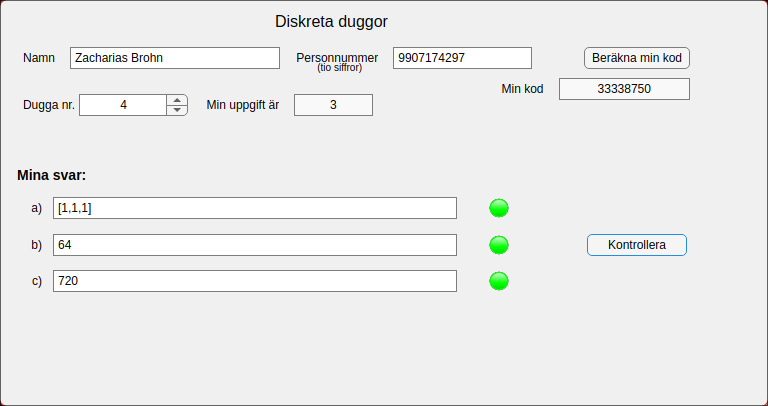
\includegraphics[width=\textwidth]{JQJzlcO.png}
\end{document}